\begin{minipage}{0.115\textwidth}
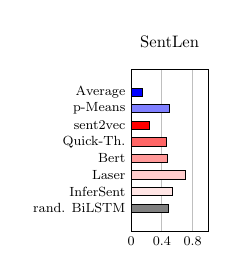
\begin{tikzpicture}[scale=0.75,every node/.style={scale=0.8}]

  	\begin{axis}[
		title=SentLen\strut,
 	   	xbar stacked,
		bar width=4pt,
		enlarge y limits=0.2,
    		symbolic y coords={rand. BiLSTM,InferSent,Laser,Bert,Quick-Th.,sent2vec,p-Means,Average},
		xmin=0,xmax=1,
  		xmajorgrids,
		tickwidth=0pt,
		xtick distance=0.40,
  		ytick=data,
		scale only axis=true,
  		width=1.3cm,height=2.75cm,
		tick label style={font=\footnotesize}
  	]

		% avg
  		\addplot[blue,fill,draw=black] coordinates
  			{(0.140,Average) (0.00,p-Means) (0.00,sent2vec) (0.00,Quick-Th.) (0.00,Bert) (0.00,Laser) (0.00,InferSent) (0.00,rand. BiLSTM)};
		% pms
		\addplot[blue!50,fill,draw=black] coordinates
			{(0.00,Average) (0.498,p-Means) (0.00,sent2vec) (0.00,Quick-Th.) (0.00,Bert) (0.00,Laser) (0.00,InferSent) (0.00,rand. BiLSTM)};

		% s2v
		\addplot[red,fill,draw=black] coordinates 
			{(0.00,Average) (0.00,p-Means) (0.240,sent2vec) (0.00,Quick-Th.) (0.00,Bert) (0.00,Laser) (0.00,InferSent) (0.00,rand. BiLSTM)};
		% qth
		\addplot[red!60,fill,draw=black] coordinates
			{(0.00,Average) (0.00,p-Means) (0.00,sent2vec) (0.454,Quick-Th.) (0.00,Bert) (0.00,Laser) (0.00,InferSent) (0.00,rand. BiLSTM)};
		% bert
		\addplot[red!40,fill,draw=black] coordinates
			{(0.00,Average) (0.00,p-Means) (0.00,sent2vec) (0.00,Quick-Th.) (0.472,Bert) (0.00,Laser) (0.00,InferSent) (0.00,rand. BiLSTM)};
		% laser
		\addplot[red!20,fill,draw=black] coordinates
			{(0.00,Average) (0.00,p-Means) (0.00,sent2vec) (0.00,Quick-Th.) (0.00,Bert) (0.705,Laser) (0.00,InferSent) (0.00,rand. BiLSTM)};
		% infersent
		\addplot[red!10,fill,draw=black] coordinates
			{(0.00,Average) (0.00,p-Means) (0.00,sent2vec) (0.00,Quick-Th.) (0.00,Bert) (0.00,Laser) (0.537,InferSent) (0.00,rand. BiLSTM)};

		% rand lstm
		\addplot[gray,fill,draw=black] coordinates 
			{(0.00,Average) (0.00,p-Means) (0.00,sent2vec) (0.00,Quick-Th.) (0.00,Bert) (0.00,Laser) (0.00,InferSent) (0.487,rand. BiLSTM)};

  	\end{axis}

\end{tikzpicture}
\end{minipage}
\hspace*{17mm}
\begin{minipage}{0.09\textwidth}
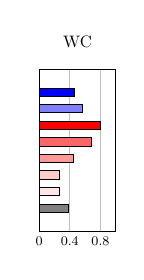
\begin{tikzpicture}[scale=0.75,every node/.style={scale=0.8}]

  	\begin{axis}[
		title=WC\strut,
   	 	xbar stacked,
		bar width=4pt,
		enlarge y limits=0.2,
	    	symbolic y coords={rand. BiLSTM,InferSent,Laser,Bert,Quick-Th.,sent2vec,p-Means,Average},
		xmin=0,xmax=1,
  		xmajorgrids,
		tickwidth=0pt,
		xtick distance=0.40,
  		ytick=data,
		yticklabels={,,},
		scale only axis=true,
  		width=1.3cm,height=2.75cm,
		tick label style={font=\footnotesize}
  	]

		% avg
  		\addplot[blue,fill,draw=black] coordinates
  			{(0.466,Average) (0.00,p-Means) (0.00,sent2vec) (0.00,Quick-Th.) (0.00,Bert) (0.00,Laser) (0.00,InferSent) (0.00,rand. BiLSTM)};
		% pms
		\addplot[blue!50,fill,draw=black] coordinates
			{(0.00,Average) (0.564,p-Means) (0.00,sent2vec) (0.00,Quick-Th.) (0.00,Bert) (0.00,Laser) (0.00,InferSent) (0.00,rand. BiLSTM)};

		% s2v
		\addplot[red,fill,draw=black] coordinates 
			{(0.00,Average) (0.00,p-Means) (0.799,sent2vec) (0.00,Quick-Th.) (0.00,Bert) (0.00,Laser) (0.00,InferSent) (0.00,rand. BiLSTM)};
		% qth
		\addplot[red!60,fill,draw=black] coordinates
			{(0.00,Average) (0.00,p-Means) (0.00,sent2vec) (0.679,Quick-Th.) (0.00,Bert) (0.00,Laser) (0.00,InferSent) (0.00,rand. BiLSTM)};
		% bert
		\addplot[red!40,fill,draw=black] coordinates
			{(0.00,Average) (0.00,p-Means) (0.00,sent2vec) (0.00,Quick-Th.) (0.446,Bert) (0.00,Laser) (0.00,InferSent) (0.00,rand. BiLSTM)};
		% laser
		\addplot[red!20,fill,draw=black] coordinates
			{(0.00,Average) (0.00,p-Means) (0.00,sent2vec) (0.00,Quick-Th.) (0.00,Bert) (0.270,Laser) (0.00,InferSent) (0.00,rand. BiLSTM)};
		% infersent
		\addplot[red!10,fill,draw=black] coordinates
			{(0.00,Average) (0.00,p-Means) (0.00,sent2vec) (0.00,Quick-Th.) (0.00,Bert) (0.00,Laser) (0.262,InferSent) (0.00,rand. BiLSTM)};

		% rand lstm
		\addplot[gray,fill,draw=black] coordinates 
			{(0.00,Average) (0.00,p-Means) (0.00,sent2vec) (0.00,Quick-Th.) (0.00,Bert) (0.00,Laser) (0.00,InferSent) (0.384,rand. BiLSTM)};

  	\end{axis}

\end{tikzpicture}
\end{minipage}
\hspace*{10mm}
\begin{minipage}{0.09\textwidth}
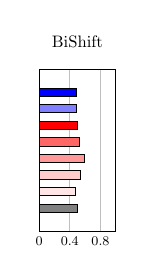
\begin{tikzpicture}[scale=0.75,every node/.style={scale=0.8}]

  	\begin{axis}[
		title=BiShift\strut,
 	   	xbar stacked,
		bar width=4pt,
		enlarge y limits=0.2,
    		symbolic y coords={rand. BiLSTM,InferSent,Laser,Bert,Quick-Th.,sent2vec,p-Means,Average},
		xmin=0,xmax=1,
  		xmajorgrids,
		tickwidth=0pt,
		xtick distance=0.40,
  		ytick=data,
		yticklabels={,,},
		scale only axis=true,
  		width=1.3cm,height=2.75cm,
		tick label style={font=\footnotesize}
  	]

		% avg
  		\addplot[blue,fill,draw=black] coordinates
  			{(0.484,Average) (0.00,p-Means) (0.00,sent2vec) (0.00,Quick-Th.) (0.00,Bert) (0.00,Laser) (0.00,InferSent) (0.00,rand. BiLSTM)};
		% pms
		\addplot[blue!50,fill,draw=black] coordinates
			{(0.00,Average) (0.487,p-Means) (0.00,sent2vec) (0.00,Quick-Th.) (0.00,Bert) (0.00,Laser) (0.00,InferSent) (0.00,rand. BiLSTM)};

		% s2v
		\addplot[red,fill,draw=black] coordinates 
			{(0.00,Average) (0.00,p-Means) (0.501,sent2vec) (0.00,Quick-Th.) (0.00,Bert) (0.00,Laser) (0.00,InferSent) (0.00,rand. BiLSTM)};
		% qth
		\addplot[red!60,fill,draw=black] coordinates
			{(0.00,Average) (0.00,p-Means) (0.00,sent2vec) (0.528,Quick-Th.) (0.00,Bert) (0.00,Laser) (0.00,InferSent) (0.00,rand. BiLSTM)};
		% bert
		\addplot[red!40,fill,draw=black] coordinates
			{(0.00,Average) (0.00,p-Means) (0.00,sent2vec) (0.00,Quick-Th.) (0.586,Bert) (0.00,Laser) (0.00,InferSent) (0.00,rand. BiLSTM)};
		% laser
		\addplot[red!20,fill,draw=black] coordinates
			{(0.00,Average) (0.00,p-Means) (0.00,sent2vec) (0.00,Quick-Th.) (0.00,Bert) (0.533,Laser) (0.00,InferSent) (0.00,rand. BiLSTM)};
		% infersent
		\addplot[red!10,fill,draw=black] coordinates
			{(0.00,Average) (0.00,p-Means) (0.00,sent2vec) (0.00,Quick-Th.) (0.00,Bert) (0.00,Laser) (0.471,InferSent) (0.00,rand. BiLSTM)};

		% rand lstm
		\addplot[gray,fill,draw=black] coordinates 
			{(0.00,Average) (0.00,p-Means) (0.00,sent2vec) (0.00,Quick-Th.) (0.00,Bert) (0.00,Laser) (0.00,InferSent) (0.503,rand. BiLSTM)};

  	\end{axis}

\end{tikzpicture}
\end{minipage}
\hspace*{10mm}
\begin{minipage}{0.09\textwidth}
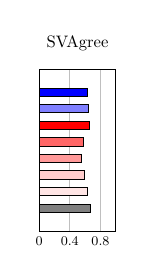
\begin{tikzpicture}[scale=0.75,every node/.style={scale=0.8}]

  	\begin{axis}[
		title=SVAgree\strut,
 	   	xbar stacked,
		bar width=4pt,
		enlarge y limits=0.2,
    		symbolic y coords={rand. BiLSTM,InferSent,Laser,Bert,Quick-Th.,sent2vec,p-Means,Average},
		xmin=0,xmax=1,
  		xmajorgrids,
		tickwidth=0pt,
		xtick distance=0.40,
  		ytick=data,
		yticklabels={,,},
		scale only axis=true,
  		width=1.3cm,height=2.75cm,
		tick label style={font=\footnotesize}
  	]

		% avg
  		\addplot[blue,fill,draw=black] coordinates
  			{(0.634,Average) (0.00,p-Means) (0.00,sent2vec) (0.00,Quick-Th.) (0.00,Bert) (0.00,Laser) (0.00,InferSent) (0.00,rand. BiLSTM)};
		% pms
		\addplot[blue!50,fill,draw=black] coordinates
			{(0.00,Average) (0.639,p-Means) (0.00,sent2vec) (0.00,Quick-Th.) (0.00,Bert) (0.00,Laser) (0.00,InferSent) (0.00,rand. BiLSTM)};

		% s2v
		\addplot[red,fill,draw=black] coordinates 
			{(0.00,Average) (0.00,p-Means) (0.650,sent2vec) (0.00,Quick-Th.) (0.00,Bert) (0.00,Laser) (0.00,InferSent) (0.00,rand. BiLSTM)};
		% qth
		\addplot[red!60,fill,draw=black] coordinates
			{(0.00,Average) (0.00,p-Means) (0.00,sent2vec) (0.579,Quick-Th.) (0.00,Bert) (0.00,Laser) (0.00,InferSent) (0.00,rand. BiLSTM)};
		% bert
		\addplot[red!40,fill,draw=black] coordinates
			{(0.00,Average) (0.00,p-Means) (0.00,sent2vec) (0.00,Quick-Th.) (0.549,Bert) (0.00,Laser) (0.00,InferSent) (0.00,rand. BiLSTM)};
		% laser
		\addplot[red!20,fill,draw=black] coordinates
			{(0.00,Average) (0.00,p-Means) (0.00,sent2vec) (0.00,Quick-Th.) (0.00,Bert) (0.590,Laser) (0.00,InferSent) (0.00,rand. BiLSTM)};
		% infersent
		\addplot[red!10,fill,draw=black] coordinates
			{(0.00,Average) (0.00,p-Means) (0.00,sent2vec) (0.00,Quick-Th.) (0.00,Bert) (0.00,Laser) (0.635,InferSent) (0.00,rand. BiLSTM)};

		% rand lstm
		\addplot[gray,fill,draw=black] coordinates 
			{(0.00,Average) (0.00,p-Means) (0.00,sent2vec) (0.00,Quick-Th.) (0.00,Bert) (0.00,Laser) (0.00,InferSent) (0.663,rand. BiLSTM)};

  	\end{axis}

\end{tikzpicture}
\end{minipage}

\vspace*{3mm}
\begin{minipage}{0.09\textwidth}
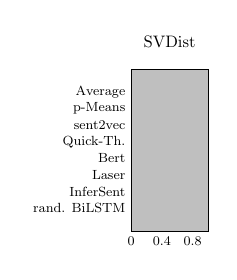
\begin{tikzpicture}[scale=0.75,every node/.style={scale=0.8}]

  	\begin{axis}[
		title=SVDist\strut,
 	   	xbar stacked,
		bar width=4pt,
		enlarge y limits=0.2,
    		symbolic y coords={rand. BiLSTM,InferSent,Laser,Bert,Quick-Th.,sent2vec,p-Means,Average},
		xmin=0,xmax=1,
  		xmajorgrids,
		tickwidth=0pt,
		xtick distance=0.40,
  		ytick=data,
		scale only axis=true,
  		width=1.3cm,height=2.75cm,
		axis background/.style={fill=lightgray},
		tick label style={font=\footnotesize}
  	]

		\addplot[blue,fill,draw=black] coordinates
  			{(0.00,Average) (0.00,p-Means) (0.00,sent2vec) (0.00,Quick-Th.) (0.00,Bert) (0.00,Laser) (0.00,InferSent) (0.00,rand. BiLSTM)};

  	\end{axis}

\end{tikzpicture}
\end{minipage}
\hspace*{19.75mm}
\begin{minipage}{0.09\textwidth}
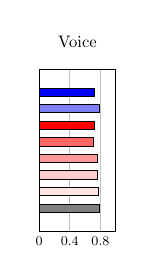
\begin{tikzpicture}[scale=0.75,every node/.style={scale=0.8}]

  	\begin{axis}[
		title=Voice\strut,
    		xbar stacked,
		bar width=4pt,
		enlarge y limits=0.2,
    		symbolic y coords={rand. BiLSTM,InferSent,Laser,Bert,Quick-Th.,sent2vec,p-Means,Average},
		xmin=0,xmax=1,
  		xmajorgrids,
		tickwidth=0pt,
		xtick distance=0.40,
  		ytick=data,
		yticklabels={,,},
		scale only axis=true,
  		width=1.3cm,height=2.75cm,
		tick label style={font=\footnotesize}
  	]

		% avg
  		\addplot[blue,fill,draw=black] coordinates
  			{(0.724,Average) (0.00,p-Means) (0.00,sent2vec) (0.00,Quick-Th.) (0.00,Bert) (0.00,Laser) (0.00,InferSent) (0.00,rand. BiLSTM)};
		% pms
		\addplot[blue!50,fill,draw=black] coordinates
			{(0.00,Average) (0.782,p-Means) (0.00,sent2vec) (0.00,Quick-Th.) (0.00,Bert) (0.00,Laser) (0.00,InferSent) (0.00,rand. BiLSTM)};

		% s2v
		\addplot[red,fill,draw=black] coordinates 
			{(0.00,Average) (0.00,p-Means) (0.726,sent2vec) (0.00,Quick-Th.) (0.00,Bert) (0.00,Laser) (0.00,InferSent) (0.00,rand. BiLSTM)};
		% qth
		\addplot[red!60,fill,draw=black] coordinates
			{(0.00,Average) (0.00,p-Means) (0.00,sent2vec) (0.707,Quick-Th.) (0.00,Bert) (0.00,Laser) (0.00,InferSent) (0.00,rand. BiLSTM)};
		% bert
		\addplot[red!40,fill,draw=black] coordinates
			{(0.00,Average) (0.00,p-Means) (0.00,sent2vec) (0.00,Quick-Th.) (0.761,Bert) (0.00,Laser) (0.00,InferSent) (0.00,rand. BiLSTM)};
		% laser
		\addplot[red!20,fill,draw=black] coordinates
			{(0.00,Average) (0.00,p-Means) (0.00,sent2vec) (0.00,Quick-Th.) (0.00,Bert) (0.765,Laser) (0.00,InferSent) (0.00,rand. BiLSTM)};
		% infersent
		\addplot[red!10,fill,draw=black] coordinates
			{(0.00,Average) (0.00,p-Means) (0.00,sent2vec) (0.00,Quick-Th.) (0.00,Bert) (0.00,Laser) (0.771,InferSent) (0.00,rand. BiLSTM)};

		% rand lstm
		\addplot[gray,fill,draw=black] coordinates 
			{(0.00,Average) (0.00,p-Means) (0.00,sent2vec) (0.00,Quick-Th.) (0.00,Bert) (0.00,Laser) (0.00,InferSent) (0.788,rand. BiLSTM)};

  	\end{axis}

\end{tikzpicture}
\end{minipage}
\hspace*{10mm}
\begin{minipage}{0.09\textwidth}
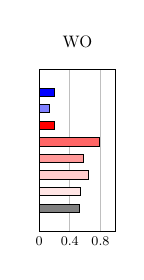
\begin{tikzpicture}[scale=0.75,every node/.style={scale=0.8}]

  	\begin{axis}[
		title=WO\strut,
   	 	xbar stacked,
		bar width=4pt,
		enlarge y limits=0.2,
    		symbolic y coords={rand. BiLSTM,InferSent,Laser,Bert,Quick-Th.,sent2vec,p-Means,Average},
		xmin=0,xmax=1,
  		xmajorgrids,
		tickwidth=0pt,
		xtick distance=0.40,
  		ytick=data,
		yticklabels={,,},
		scale only axis=true,
  		width=1.3cm,height=2.75cm,
		tick label style={font=\footnotesize}
  	]

		% avg
  		\addplot[blue,fill,draw=black] coordinates
  			{(0.195,Average) (0.00,p-Means) (0.00,sent2vec) (0.00,Quick-Th.) (0.00,Bert) (0.00,Laser) (0.00,InferSent) (0.00,rand. BiLSTM)};
		% pms
		\addplot[blue!50,fill,draw=black] coordinates
			{(0.00,Average) (0.139,p-Means) (0.00,sent2vec) (0.00,Quick-Th.) (0.00,Bert) (0.00,Laser) (0.00,InferSent) (0.00,rand. BiLSTM)};

		% s2v
		\addplot[red,fill,draw=black] coordinates 
			{(0.00,Average) (0.00,p-Means) (0.206,sent2vec) (0.00,Quick-Th.) (0.00,Bert) (0.00,Laser) (0.00,InferSent) (0.00,rand. BiLSTM)};
		% qth
		\addplot[red!60,fill,draw=black] coordinates
			{(0.00,Average) (0.00,p-Means) (0.00,sent2vec) (0.787,Quick-Th.) (0.00,Bert) (0.00,Laser) (0.00,InferSent) (0.00,rand. BiLSTM)};
		% bert
		\addplot[red!40,fill,draw=black] coordinates
			{(0.00,Average) (0.00,p-Means) (0.00,sent2vec) (0.00,Quick-Th.) (0.584,Bert) (0.00,Laser) (0.00,InferSent) (0.00,rand. BiLSTM)};
		% laser
		\addplot[red!20,fill,draw=black] coordinates
			{(0.00,Average) (0.00,p-Means) (0.00,sent2vec) (0.00,Quick-Th.) (0.00,Bert) (0.640,Laser) (0.00,InferSent) (0.00,rand. BiLSTM)};
		% infersent
		\addplot[red!10,fill,draw=black] coordinates
			{(0.00,Average) (0.00,p-Means) (0.00,sent2vec) (0.00,Quick-Th.) (0.00,Bert) (0.00,Laser) (0.543,InferSent) (0.00,rand. BiLSTM)};

		% rand lstm
		\addplot[gray,fill,draw=black] coordinates 
			{(0.00,Average) (0.00,p-Means) (0.00,sent2vec) (0.00,Quick-Th.) (0.00,Bert) (0.00,Laser) (0.00,InferSent) (0.525,rand. BiLSTM)};

  	\end{axis}

\end{tikzpicture}
\end{minipage}
\hspace*{10mm}
\begin{minipage}{0.09\textwidth}
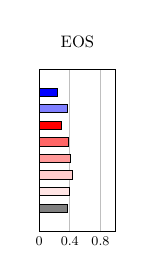
\begin{tikzpicture}[scale=0.75,every node/.style={scale=0.8}]

  	\begin{axis}[
		title=EOS\strut,
  	  	xbar stacked,
		bar width=4pt,
		enlarge y limits=0.2,
    		symbolic y coords={rand. BiLSTM,InferSent,Laser,Bert,Quick-Th.,sent2vec,p-Means,Average},
		xmin=0,xmax=1,
  		xmajorgrids,
		tickwidth=0pt,
		xtick distance=0.40,
  		ytick=data,
		yticklabels={,,},
		scale only axis=true,
  		width=1.3cm,height=2.75cm,
		tick label style={font=\footnotesize}
  	]

		% avg
  		\addplot[blue,fill,draw=black] coordinates
  			{(0.241,Average) (0.00,p-Means) (0.00,sent2vec) (0.00,Quick-Th.) (0.00,Bert) (0.00,Laser) (0.00,InferSent) (0.00,rand. BiLSTM)};
		% pms
		\addplot[blue!50,fill,draw=black] coordinates
			{(0.00,Average) (0.366,p-Means) (0.00,sent2vec) (0.00,Quick-Th.) (0.00,Bert) (0.00,Laser) (0.00,InferSent) (0.00,rand. BiLSTM)};

		% s2v
		\addplot[red,fill,draw=black] coordinates 
			{(0.00,Average) (0.00,p-Means) (0.294,sent2vec) (0.00,Quick-Th.) (0.00,Bert) (0.00,Laser) (0.00,InferSent) (0.00,rand. BiLSTM)};
		% qth
		\addplot[red!60,fill,draw=black] coordinates
			{(0.00,Average) (0.00,p-Means) (0.00,sent2vec) (0.387,Quick-Th.) (0.00,Bert) (0.00,Laser) (0.00,InferSent) (0.00,rand. BiLSTM)};
		% bert
		\addplot[red!40,fill,draw=black] coordinates
			{(0.00,Average) (0.00,p-Means) (0.00,sent2vec) (0.00,Quick-Th.) (0.413,Bert) (0.00,Laser) (0.00,InferSent) (0.00,rand. BiLSTM)};
		% laser
		\addplot[red!20,fill,draw=black] coordinates
			{(0.00,Average) (0.00,p-Means) (0.00,sent2vec) (0.00,Quick-Th.) (0.00,Bert) (0.435,Laser) (0.00,InferSent) (0.00,rand. BiLSTM)};
		% infersent
		\addplot[red!10,fill,draw=black] coordinates
			{(0.00,Average) (0.00,p-Means) (0.00,sent2vec) (0.00,Quick-Th.) (0.00,Bert) (0.00,Laser) (0.393,InferSent) (0.00,rand. BiLSTM)};

		% rand lstm
		\addplot[gray,fill,draw=black] coordinates 
			{(0.00,Average) (0.00,p-Means) (0.00,sent2vec) (0.00,Quick-Th.) (0.00,Bert) (0.00,Laser) (0.00,InferSent) (0.368,rand. BiLSTM)};

  	\end{axis}

\end{tikzpicture}
\end{minipage}
\hspace*{10mm}
\begin{minipage}{0.09\textwidth}
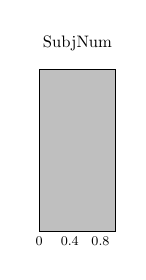
\begin{tikzpicture}[scale=0.75,every node/.style={scale=0.8}]

  	\begin{axis}[
		title=SubjNum\strut,
    		xbar stacked,
		bar width=4pt,
		enlarge y limits=0.2,
    		symbolic y coords={rand. BiLSTM,InferSent,Laser,Bert,Quick-Th.,sent2vec,p-Means,Average},
		xmin=0,xmax=1,
  		xmajorgrids,
		tickwidth=0pt,
		xtick distance=0.40,
  		ytick=data,
		yticklabels={,,},
		scale only axis=true,
  		width=1.3cm,height=2.75cm,
		axis background/.style={fill=lightgray},
		tick label style={font=\footnotesize}
  	]

		\addplot[blue,fill,draw=black] coordinates
  			{(0.00,Average) (0.00,p-Means) (0.00,sent2vec) (0.00,Quick-Th.) (0.00,Bert) (0.00,Laser) (0.00,InferSent) (0.00,rand. BiLSTM)};

  	\end{axis}

\end{tikzpicture}
\end{minipage}